\documentclass[border=5pt]{standalone}
\usepackage{pgfplots}

\begin{document}
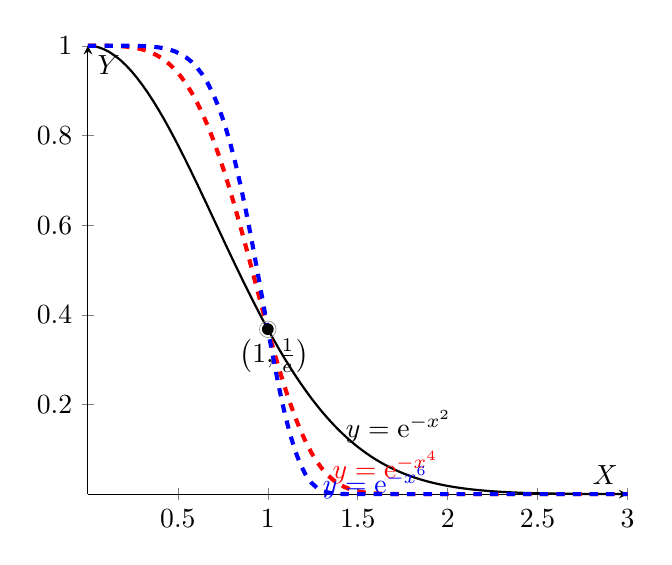
\begin{tikzpicture}
    \begin{axis}[
        axis lines=center,
        xlabel=$X$,
        ylabel=$Y$,
        legend style={at={(0.97,0.3)}, anchor=east},
        ymin=0, ymax=1,
        xmin=0, xmax=3,
        samples=100,
        domain=0:3,
        clip=false,
        ]
        
        \addplot[thick, mark=none] {exp(-x^2)} node[pos=0.5, right] {$y=\mathrm{e}^{-x^2}$};
        \addplot[thick, mark=none, dashed, red, line width=1.5pt] {exp(-x^4)} node[pos=0.5, right] {$y=\mathrm{e}^{-x^4}$};
        \addplot[thick, mark=none, dashed, blue, line width=1.5pt] {exp(-x^6)} node[pos=0.5, right] {$y=\mathrm{e}^{-x^6}$};
        
        \node[circle,fill,inner sep=1.5pt,label={[anchor=north]right:$\left(1,\frac{1}{e}\right)$}] at (axis cs:1,{exp(-1)}) {};
        \draw[very thin,gray] (axis cs:1,{exp(-1)}) circle (3pt);
        
    \end{axis}
\end{tikzpicture}
\end{document}